\chapter{Referencial Teórico}
\label{ch:referencial}

Neste capítulo é apresentada a fundamentação teórica deste trabalho, abordando conceitos e metodologias e facilitando a compreensão das tomadas de decisão que construíram a proposta de estudo apresentada no Capítulo \ref{ch:proposta}.

\section{Experimentação na Engenharia de Software}
\label{subsec:experimentacao}

A experimentação é um domínio fundamental da investigação empírica, oferecendo uma abordagem disciplinada e quantificável para a análise de fenômenos de interesse. Na engenharia de software, essa abordagem é crucial, pois trata-se de uma área multidisciplinar que depende diretamente da avaliação da atividade humana. A pesquisa científica se torna especialmente relevante em momentos de tomada de decisão sobre como softwares são desenvolvidos, contribuindo para o avanço do conhecimento por meio da avaliação das atividades realizadas por pessoas em seus diferentes contextos \cite{wohlin_experimentation_2012}.

\citeonline{basili_experimental_1993} apresentou quatro métodos de pesquisa na Engenharia de \textit{Software}: \textit{Scientific}, \textit{Engineering}, \textit{Empirical} e \textit{Analytical}. Dentre eles, o método Empírico (\textit{Empirical}) é amplamente utilizado em ciências sociais e psicologia para estudar o comportamento humano em contextos onde leis formais não se aplicam, sendo igualmente aplicável à Engenharia de \textit{Software} quando se é necessário lidar com aspectos que não são puramente técnicos \cite{wohlin_experimentation_2012}.

Entre as estratégias de investigação empírica está o \textbf{Estudo de Caso}, que utiliza diversas fontes de dados para investigar um fenômeno em seu contexto real. Este método avalia o caso em questão de forma quantitativa ou qualitativa, sem intervenção ou controle, sendo, portanto, um estudo observacional \cite{runeson_case_study_2012}.

Outra estratégia é o \textbf{Experimento}, que, ao contrário do estudo de caso, busca um controle sistemático e direto sobre a situação estudada. Para isto, identifica o contexto de interesse e coleta amostras de variáveis para validar teorias, confirmar ou explorar relacionamentos. É normalmente utilizado quando o objetivo é comparar diferentes tratamentos para uma mesma situação \cite{wohlin_experimentation_2012}.

Utilizada no contexto deste trabalho, há também a \textbf{Revisão Sistemática da Literatura}, que busca reunir evidências empíricas de diversas fontes literárias através de buscas em portais, bancos de dados acadêmicos ou outras fontes. Dessa forma, através do seu protocolo, é possível sintetizar o estado da arte do domínio desejado por meio de uma avaliação sistemática das informações encontradas na literatura \cite{kitchenham_rsl}.

\todo[inline, color=pink]{Salvo engano eu havia feito um comentário nesse semtido. Essa introdução ficou restrita. Por mais que você detalhe os métodos que você vai utilizar, nessa introdução, precisa apararecer uma visão geral. Tipo o cap.2  do Wohlin. Por exemplo, flatou falar de survey/questionário, pesquisa-ação, estudos etnográficos...}


\subsection{Experimento}

Este método de investigação permite a exploração e validação de relacionamentos através de testes de hipótese e análises estatísticas. Seguindo o apresentado por \citeonline{wohlin_experimentation_2012}, serão apresentados os principais artefatos envolvidos neste processo, bem como as etapas necessárias para sua realização.

\subsubsection{Artefatos}

\begin{itemize}
    \item \textbf{Variáveis}: ao conduzir um experimento, se observa o comportamento de determinadas variáveis durante o processo escolhido. Aquelas que são alteradas para gerar os resultados são chamadas de \textbf{variáveis independentes}, ou \textbf{fatores}. Já aquelas que são responsáveis por informar os efeitos encontrados, são as \textbf{variáveis dependentes};
    \item \textbf{Tratamentos}: valor particular e específico aplicado a um fator. Cada tratamento representa uma configuração particular que é testada no experimento;
    \item \textbf{Objetos}: são os elementos ou itens sobre os quais os tratamentos são aplicados e avaliados, ou seja, quaisquer artefatos ou processos que estejam sendo estudados ou testados, e
    \item \textbf{Sujeitos}: participantes do experimento. Aqueles que são expostos aos diferentes tratamentos.
\end{itemize}

\subsubsection{Processo}

\begin{itemize}
    \item \textbf{Definição de Escopo:} onde se define claramente o problema, os objetivos e as metas do estudo. É crucial estabelecer o escopo para direcionar adequadamente o experimento, o que inclui a formulação inicial da hipótese, a definição do objeto de estudo, o propósito, o foco de qualidade, a perspectiva e o seu contexto;
    \item \textbf{Planejamento:} nesta fase são elaborados os detalhes necessários para a execução do estudo. A hipótese a ser testada é formalizada, são indetificadas as variáveis independentes e dependentes, escolhe-se o \textit{design} do experimento e são preparados os instrumentos necessários. É importante determinar os valores das variáveis e preparar os objetos de estudo, assim como desenvolver diretrizes para a coleta de dados e avaliar a validade dos resultados esperados;
    \item \textbf{Operação:} condução efetiva do experimento. Esta fase inclui a preparação dos sujeitos e materiais, a execução do experimento conforme o planejamento e a validação dos dados coletados para garantir que são corretos e representativos. A execução deve seguir o plano estabelecido para assegurar a integridade dos resultados;
    \item \textbf{Análise e Interpretação:} envolve analisar e interpretar os dados coletados. Utiliza-se estatísticas descritivas para compreender os dados e realiza-se testes de hipótese para avaliar a relação entre as variáveis. A análise pode incluir a redução de dados e a interpretação dos resultados, ajudando a validar as conclusões do experimento;
    \item \textbf{Apresentação e Empacotamento:} concentra-se na documentação e apresentação dos resultados do experimento. O objetivo é comunicar os achados de forma clara e eficaz, o que pode incluir a preparação de relatórios, a publicação dos resultados e a criação de pacotes de laboratório para facilitar a replicação do estudo. Uma documentação completa e detalhada é essencial para garantir que os resultados possam ser replicados e utilizados para futuras pesquisas.
\end{itemize}


\subsection{Estudo de Caso}

Permite uma compreensão aprofundada e contextualizada dos fenômenos de interesse através de investigações dentro de seus contextos reais. Além disso, é flexível, o que possibilita ajustes iterativos em diferentes momentos do processo. A seguir, serão definidas suas etapas de realização: definição, preparação e coleta de dados, análise de dados e relato dos resultados \cite{yin_case_study_2009}.

\subsubsection{Definição}

Segundo \citeonline{wohlin_experimentation_2012}, é a etapa inicial, nela são definidas as bases da pesquisa, através do levantamento dos seguintes artefatos:

\begin{itemize}
    \item \textbf{Objetivo:} inicialmente, é formulado de forma genérica, com um foco principal que será refinado ao longo do estudo. Define o que o pesquisador pretende alcançar e as perguntas que guiarão a investigação;
    \item \textbf{Caso:} definição do objeto de estudo da pesquisa. Pode ser um projeto, um processo, um grupo de pessoas, ou qualquer outro fenômeno que esteja sendo investigado. O caso deve necessariamente ser observado em seu contexto real, permitindo que o pesquisador capture as complexidades e nuances do ambiente;
    \item \textbf{Trabalhos Relacionados:} resultado de uma revisão sobre o estado geral da área de conhecimento à ser estudada, visando pontos de partida em outros trabalhos. Ajuda a identificar lacunas de pesquisa, construir o referencial teórico e fornecer embasamento para a formulação das questões de pesquisa;
    \item \textbf{Questões de Pesquisa:} devem ser claras e orientadoras. Funcionam como um norte para o estudo, direcionando o processo de coleta e análise de dados. Perguntas bem formuladas garantem que o estudo permaneça focado e relevante, abordando as principais preocupações do fenômeno em análise;
    \item \textbf{Métodos:} abordagem de coletas de dados à serem adotadas, dependem das questões de pesquisa e do contexto. A definição clara dos métodos contribui para a validade e confiabilidade do estudo. E
    \item \textbf{Seleção:} refere-se à escolha das fontes de dados e dos participantes do estudo. É crucial que essas escolhas sejam feitas de maneira consciente, considerando a relevância e representatividade das fontes em relação ao objetivo do estudo.
\end{itemize}

\subsubsection{Preparação e Coleta de Dados}
Aqui, o pesquisador deve estruturar cuidadosamente o processo, garantindo que os dados coletados sejam pertinentes e válidos. \citeonline{wohlin_experimentation_2012} destacam a importância da triangulação, que envolve o uso de múltiplas fontes de dados para fortalecer a validade dos resultados. 

A coleta de dados é uma etapa crítica e pode ocorrer de maneira contínua ao longo do estudo. A combinação de diferentes métodos e fontes de dados fortalece a pesquisa e proporciona uma visão mais abrangente do fenômeno. De acordo com \citeonline{lethbridge2005studying},  as técnicas de coleta de dados são divididas em três graus:

\begin{itemize}
    \item \textbf{Primeiro Grau:} técnicas que exigem contato direto com os participantes, como entrevistas, questionários e grupos de discussão. Essas técnicas fornecem dados ricos e detalhados, mas exigem maior envolvimento do pesquisador e podem ser mais caras e demoradas.
    
    \item \textbf{Segundo Grau:} envolve a observação direta do ambiente de estudo sem interação com os participantes. Exemplos incluem a observação do trabalho de uma equipe ou a coleta de métricas de um sistema em funcionamento. Essas técnicas permitem captar o comportamento natural dos participantes, mas podem ser limitadas em termos de profundidade.
    
    \item \textbf{Terceiro Grau:} utiliza dados já existentes, como documentação e registros históricos. Embora menos intrusivos, esses métodos podem ser limitados pela qualidade e relevância dos dados disponíveis. No entanto, são úteis para complementar as técnicas de primeiro e segundo grau.
\end{itemize}

\subsubsection{Análise de Dados}

Processo de interpretação e  busca de padrões nos dados coletados, e que permite ao pesquisador identificar as relações entre as variáveis e os resultados observados \cite{yin_case_study_2009}. Segundo \citeonline{wohlin_experimentation_2012}, a análise de dados pode ser realizada por meio de técnicas qualitativas, quantitativas ou uma combinação de ambas, dependendo da natureza dos dados e dos objetivos da pesquisa.

Para garantir uma análise robusta, \citeonline{wohlin_experimentation_2012} sugerem a adoção de estratégias de categorização dos dados, onde os dados são organizados em categorias ou temas, facilitando a identificação de padrões e a construção de teorias baseadas nas evidências empíricas. O uso de software de análise qualitativa pode ser útil para codificar e categorizar grandes volumes de dados textuais.

Além disso, a análise de dados pode incluir a verificação de validade interna e a validação cruzada dos resultados, assegurando que as conclusões não sejam apenas fruto de coincidências ou de vieses do pesquisador, mas que realmente representem o fenômeno estudado \cite{yin_case_study_2009}.

\subsubsection{Relato}

\citeonline{robson2002real} destaca que o relato é essencial não apenas para comunicar os resultados da pesquisa, mas também para permitir a avaliação da qualidade do estudo por parte de outros pesquisadores, e que, para isto, deve abordar os seguintes aspectos:

\begin{itemize}
\item \textbf{Contexto:} Descrição detalhada do ambiente em que o estudo foi conduzido, incluindo informações sobre os participantes, o período e as condições específicas que podem ter influenciado os resultados. Essa seção deve permitir ao leitor compreender as particularidades do caso estudado, ajudando a contextualizar os resultados.

\item \textbf{Procedimentos:} Explicação das etapas seguidas ao longo do estudo, desde a definição do caso até a coleta e análise dos dados. A clareza na descrição dos procedimentos garante a transparência metodológica, permitindo que outros pesquisadores avaliem a robustez do estudo e, eventualmente, o repliquem.

\item \textbf{Resultados:} Apresentação dos achados de forma estruturada, utilizando ferramentas como tabelas, gráficos e citações diretas dos participantes, quando aplicável, para ilustrar os pontos principais. Deve-se fornecer "instantâneos" relevantes dos dados coletados que sustentem as conclusões apresentadas, garantindo uma cadeia de evidências sólida.

\item \textbf{Discussão:} Interpretação dos resultados à luz da literatura existente, identificando as contribuições do estudo, suas limitações e as implicações práticas ou teóricas. A discussão deve situar os achados no contexto mais amplo do campo de estudo, explorando como eles se relacionam com pesquisas anteriores e quais novas questões surgem a partir das descobertas.

\item \textbf{Conclusões:} Resumo das principais descobertas e sugestões para pesquisas futuras. As conclusões devem sintetizar as contribuições do estudo e indicar como ele avança o conhecimento na área, além de propor direções para estudos subsequentes.
\end{itemize}

 
\section{\textit{Lean Startup}}

Esta metodologia \cite{ries2011lean} propõe uma abordagem contínua e sistemática de inovação sob a perspectiva das \textit{startups}, seu pensamento pode ser resumido em sete princípios: otimizar o todo, eliminar desperdícios, entregar valor, aprender constantemente, entregar rapidamente, engajar todos os participantes e melhorar continuamente \cite{poppendieck2003lean}. 


Para isso, o autor propõe um ciclo de aprendizado contínuo chamado \textit{Build-Measure-Learn}, para melhor compreensão dos desejos e das necessidades dos clientes. A fase de \textit{Build} foca na construção da funcionalidade, enquanto a fase de \textit{Measure} concentra-se na instrumentação dos dados de comportamento do usuário no sistema. Por fim, a fase de \textit{Learning} tem como objetivo usar os dados coletados para entender como as hipóteses e suposições foram realmente recebidas após a \textit{release}, a fim de construir um corpo de conhecimento sobre o produto e fomentar um ambiente de contínua inovação.

\section{\textit{Online Controlled Experiment}}

Também conhecido como Teste A/B ou simplesmente \textit{OCE}, é um experimento realizado no contexto \textit{online}. Esse tipo de investigação tem como objetivo analisar diferentes versões de \textit{software}, escolhendo métricas para comparar variantes de uma mesma funcionalidade e validar ideias sobre o desenvolvimento do produto (e.g., dispor os elementos de maneira diferente em uma página \textit{web} deve tornar determinada atividade mais rápida). A versão inicial, sem mudanças, é chamada de controle, e a atualizada, de tratamento \cite{fabijan_online_2020}.

Durante a utilização, os usuários são distribuídos entre essas diferentes versões, e, à medida que interagem com o produto, suas atividades são registradas e as métricas escolhidas são coletadas. A diferença entre esses valores, caso seja estatisticamente significativa e se a coleta de dados foi feita corretamente, muito provavelmente foi introduzida pelo tratamento \cite{kohavi_oce_and_ab_tests_2017}. Dessa forma, finaliza-se um fluxo contínuo de aprendizado, semelhante ao ciclo proposto pela metodologia \textit{Lean}. Esse ciclo já foi formalizado anteriormente na literatura e é apresentado na Figura \ref{fig:oce_lifecycle}.

\begin{figure}
    \centering
    \caption{\textit{The Experiment Lifecycle} }
    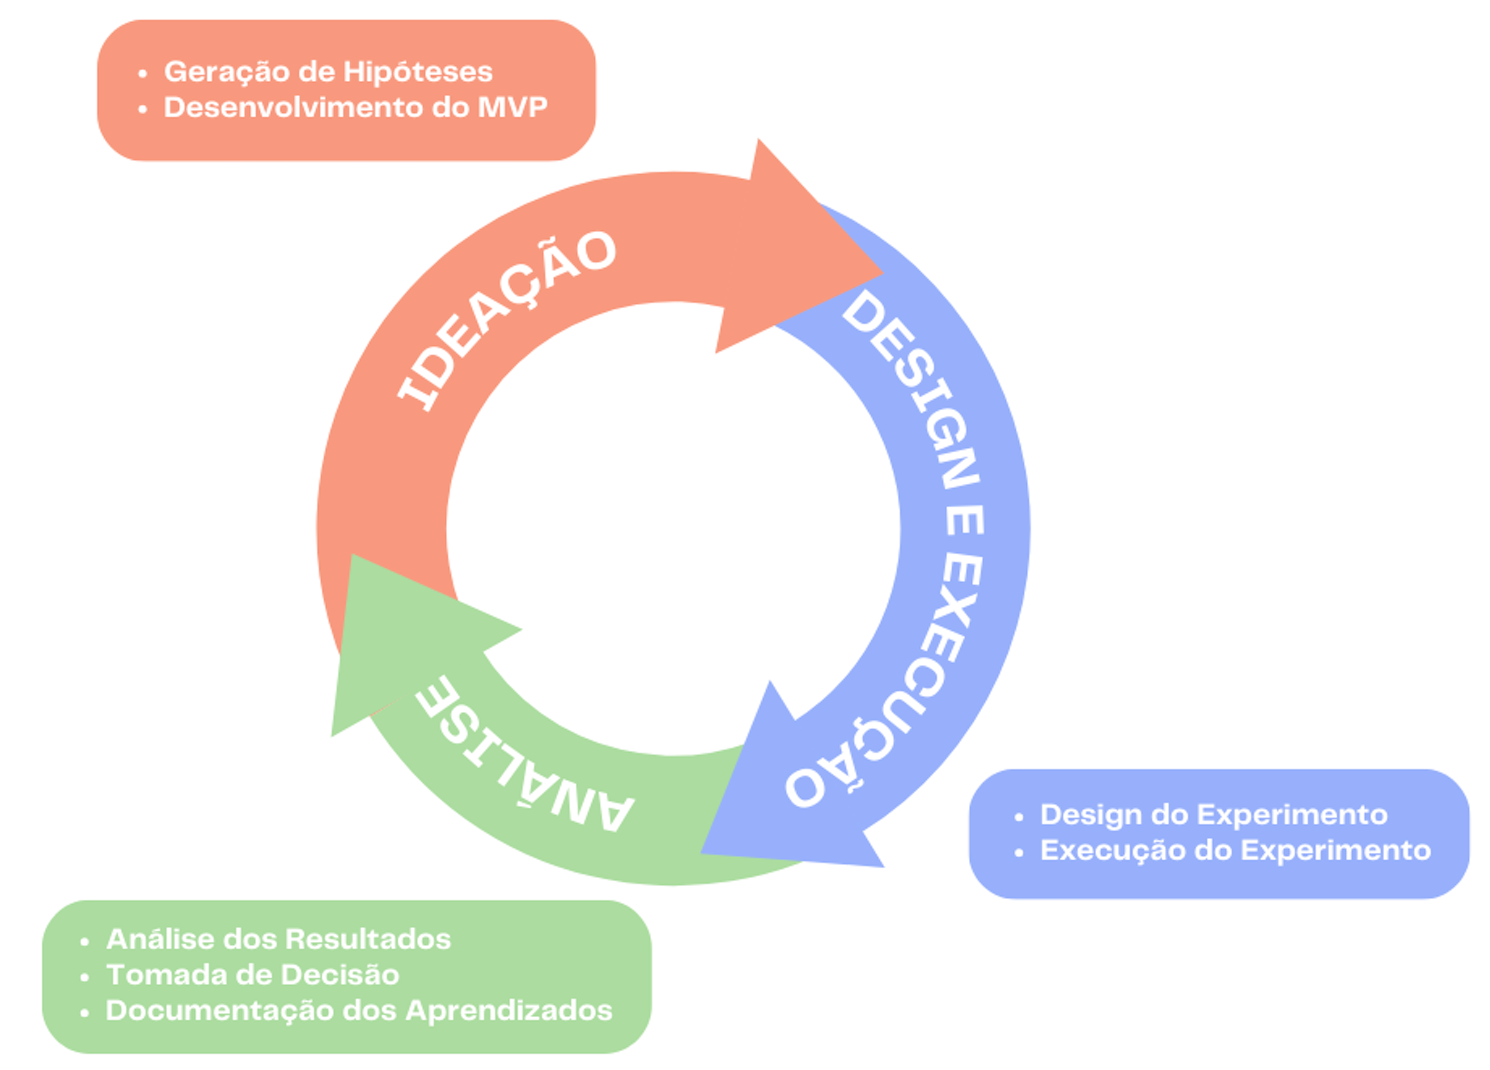
\includegraphics[width=0.75\linewidth]{figuras/oce_lifecycle.png}
    \text{Fonte: Adaptado de \citeonline{kohavi_online_2013}}
    \label{fig:oce_lifecycle}
\end{figure}

\section{\textit{Feature Toggles}}
\label{sec:ref-feature-toggle}

Nos últimos anos, empresas de \textit{software} têm priorizado cada vez mais a entrega contínua de funcionalidades para os seus usuários, diminuindo o tempo entre \textit{releases} \cite{humble_farley_2010}. Com isso, o processo de integração se torna mais complexo, já que é necessário unir diferentes entregas de diversas equipes de desenvolvedores a fim de gerar uma nova versão funcional e estável do produto \cite{berczuk_appleton_2002}.

Por ser um processo complicado, diversas soluções já surgiram no mercado; uma delas é a arquitetura de \textit{Feature Toggles} (também conhecidos como \textit{feature gates} ou \textit{feature flags}). Esta solução é um conceito simples: variáveis condicionais que envolvem determinados blocos de código, podendo ser habilitadas ou desabilitadas dependendo do contexto (por exemplo, ativar apenas para testes internos ou usuários beta). Essa abordagem em aplicações modernas permite que funcionalidades sejam ligadas ou desligadas em tempo de execução no lado do cliente, sem a necessidade de uma nova compilação \cite{rahman_feature_toggle_2016}.

Uma das desvantagens da utilização dessas \textit{flags} é a dívida técnica que elas geram, já que, uma vez que a funcionalidade tenha sido testada e liberada para a base total de usuários, a parte remanescente do código se torna obsoleta e inutilizada \cite{rahman_feature_toggle_2016}. Apesar disso, por viabilizar a divisão dos usuários entre versões diferentes de funcionalidades, esta arquitetura se mostra uma possível maneira de realizar experimentos e já é uma prática utilizada no mercado \cite{issa_mattos_hurrier_2023}.

\section{Qualidade de Software}

A qualidade do \textit{software} é um aspecto fundamental que impacta diretamente a eficácia do sistema em seu contexto de uso \citeonline{iso25000}. A norma \citeonline{iso25000} define a qualidade do produto de \textit{software} em termos de características e subcaracterísticas que determinam sua capacidade de satisfazer as necessidades explícitas e implícitas dos usuários. Além disso, a qualidade em uso refere-se ao efeito percebido pelo usuário final ao interagir com o \textit{software} em seu ambiente operacional.

A avaliação da qualidade de um produto de \textit{software} em uso é essencial para garantir que o sistema não apenas funcione conforme especificado, mas também atenda às expectativas e requisitos dos usuários em situações reais de operação. As características e subcaracterísticas da qualidade em uso são definidas pela norma \citeonline{iso25010} e são apresentadas na Figura \ref{fig:quality-in-use}.

\begin{figure}[h]
\centering
\caption{Modelo de Qualidade em Uso}
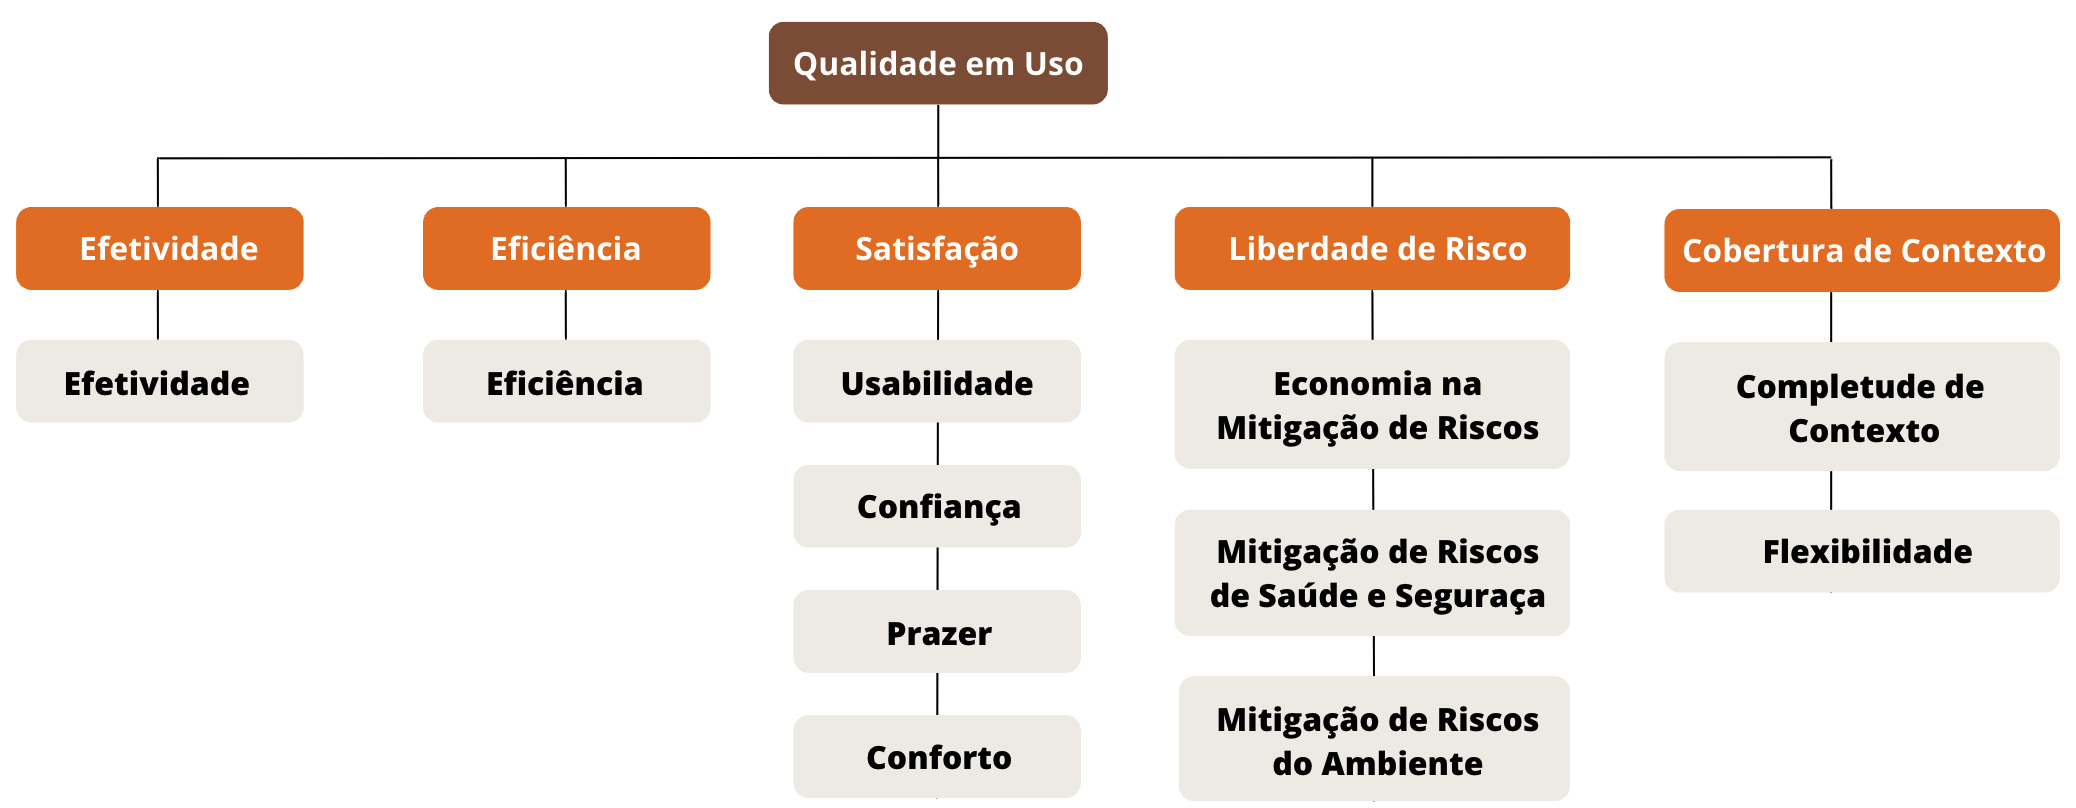
\includegraphics[width=1\linewidth]{figuras/quality_in_use.png}
\text{Fonte: Norma \citeonline{iso25010}}
\label{fig:quality-in-use}
\end{figure}

O foco desta monografia está na característica de qualidade de \textbf{eficácia}. A eficácia refere-se à precisão e à completude com que o \textit{software} permite que os usuários alcancem os objetivos esperados. A norma \citeonline{iso9241} define que, para avaliar determinada característica, devem ser definidas medidas de critério para tal, e exemplifica que, em termos de eficácia, estas devem estar relacionadas a quantidade de vezes que uma tarefa é realizada com sucesso, garantindo que o usuário alcançou seus objetivos específicos.

Os experimentos controlados visam, dentre outros objetivos, aumentar a qualidade do \textit{software}, entregando apenas as funcionalidades que realmente agregam valor para o usuário \cite{fabijan_online_2020}. As métricas observadas no momento de avaliar o tratamento em um experimento são escolhidas para validar se os usuários realmente preferem a nova versão, o que pode ser interpretado como nível de eficácia da variante.

\section{Experimentação Contínua}
\label{sec:ref-experimentacao-continua}

Na literatura, a Experimentação Contínua (ou \textit{Continuous Experimentation}, \textit{CE}) recebe diferentes denominações, como desenvolvimento orientado a dados (\textit{Data-Driven Development}), sistema de inovação experimental, entre outras \cite{erthal_characterization_2023}. Esses termos normalmente se referem ao mesmo conceito: a definição sistemática de hipóteses, entrega contínua e monitoramento de métricas para avaliação de ideias com base em evidências do uso do \textit{software} em seu contexto real \cite{fagerholm_right_2017}.

Essa prática surgiu no contexto fortemente influenciado pela metodologia \textit{Lean} e tem se tornado cada vez mais comum no mercado, sendo adotada por grandes organizações como Facebook, Google e Microsoft \cite{issa_mattos_hurrier_2023}. Diversos benefícios já foram apresentados na literatura, como aumentar a probabilidade de atender às expectativas dos usuários e aumentar seu engajamento, prevenindo o abandono do serviço, o que pode impactar significativamente a receita anual de um produto \cite{erthal_characterization_2023}.

Apesar de todos os seus benefícios, implementar um sistema de experimentação contínua pode ser desafiador, dado que, além dos testes A/B, esse processo envolve diversas outras atividades e técnicas que conectam os níveis estratégico e de desenvolvimento \cite{issa_mattos_hurrier_2023}. \citeonline{erthal_characterization_2023} apresenta uma revisão da literatura visando caracterizar essas atividades, visto que não há um consenso sobre elas e, normalmente, cada companhia as executa de forma particular. Os autores reuniram e combinaram os diferentes modelos e processos encontrados na literatura e criaram um diagrama que visa descrever as principais atividades a serem realizadas em um sistema de experimentação contínua. Este modelo é apresentado na Figura \ref{fig:erthal-process}.

\begin{figure}
\centering
\caption{\textit{A Combined Process for Continuous Experimentation}}
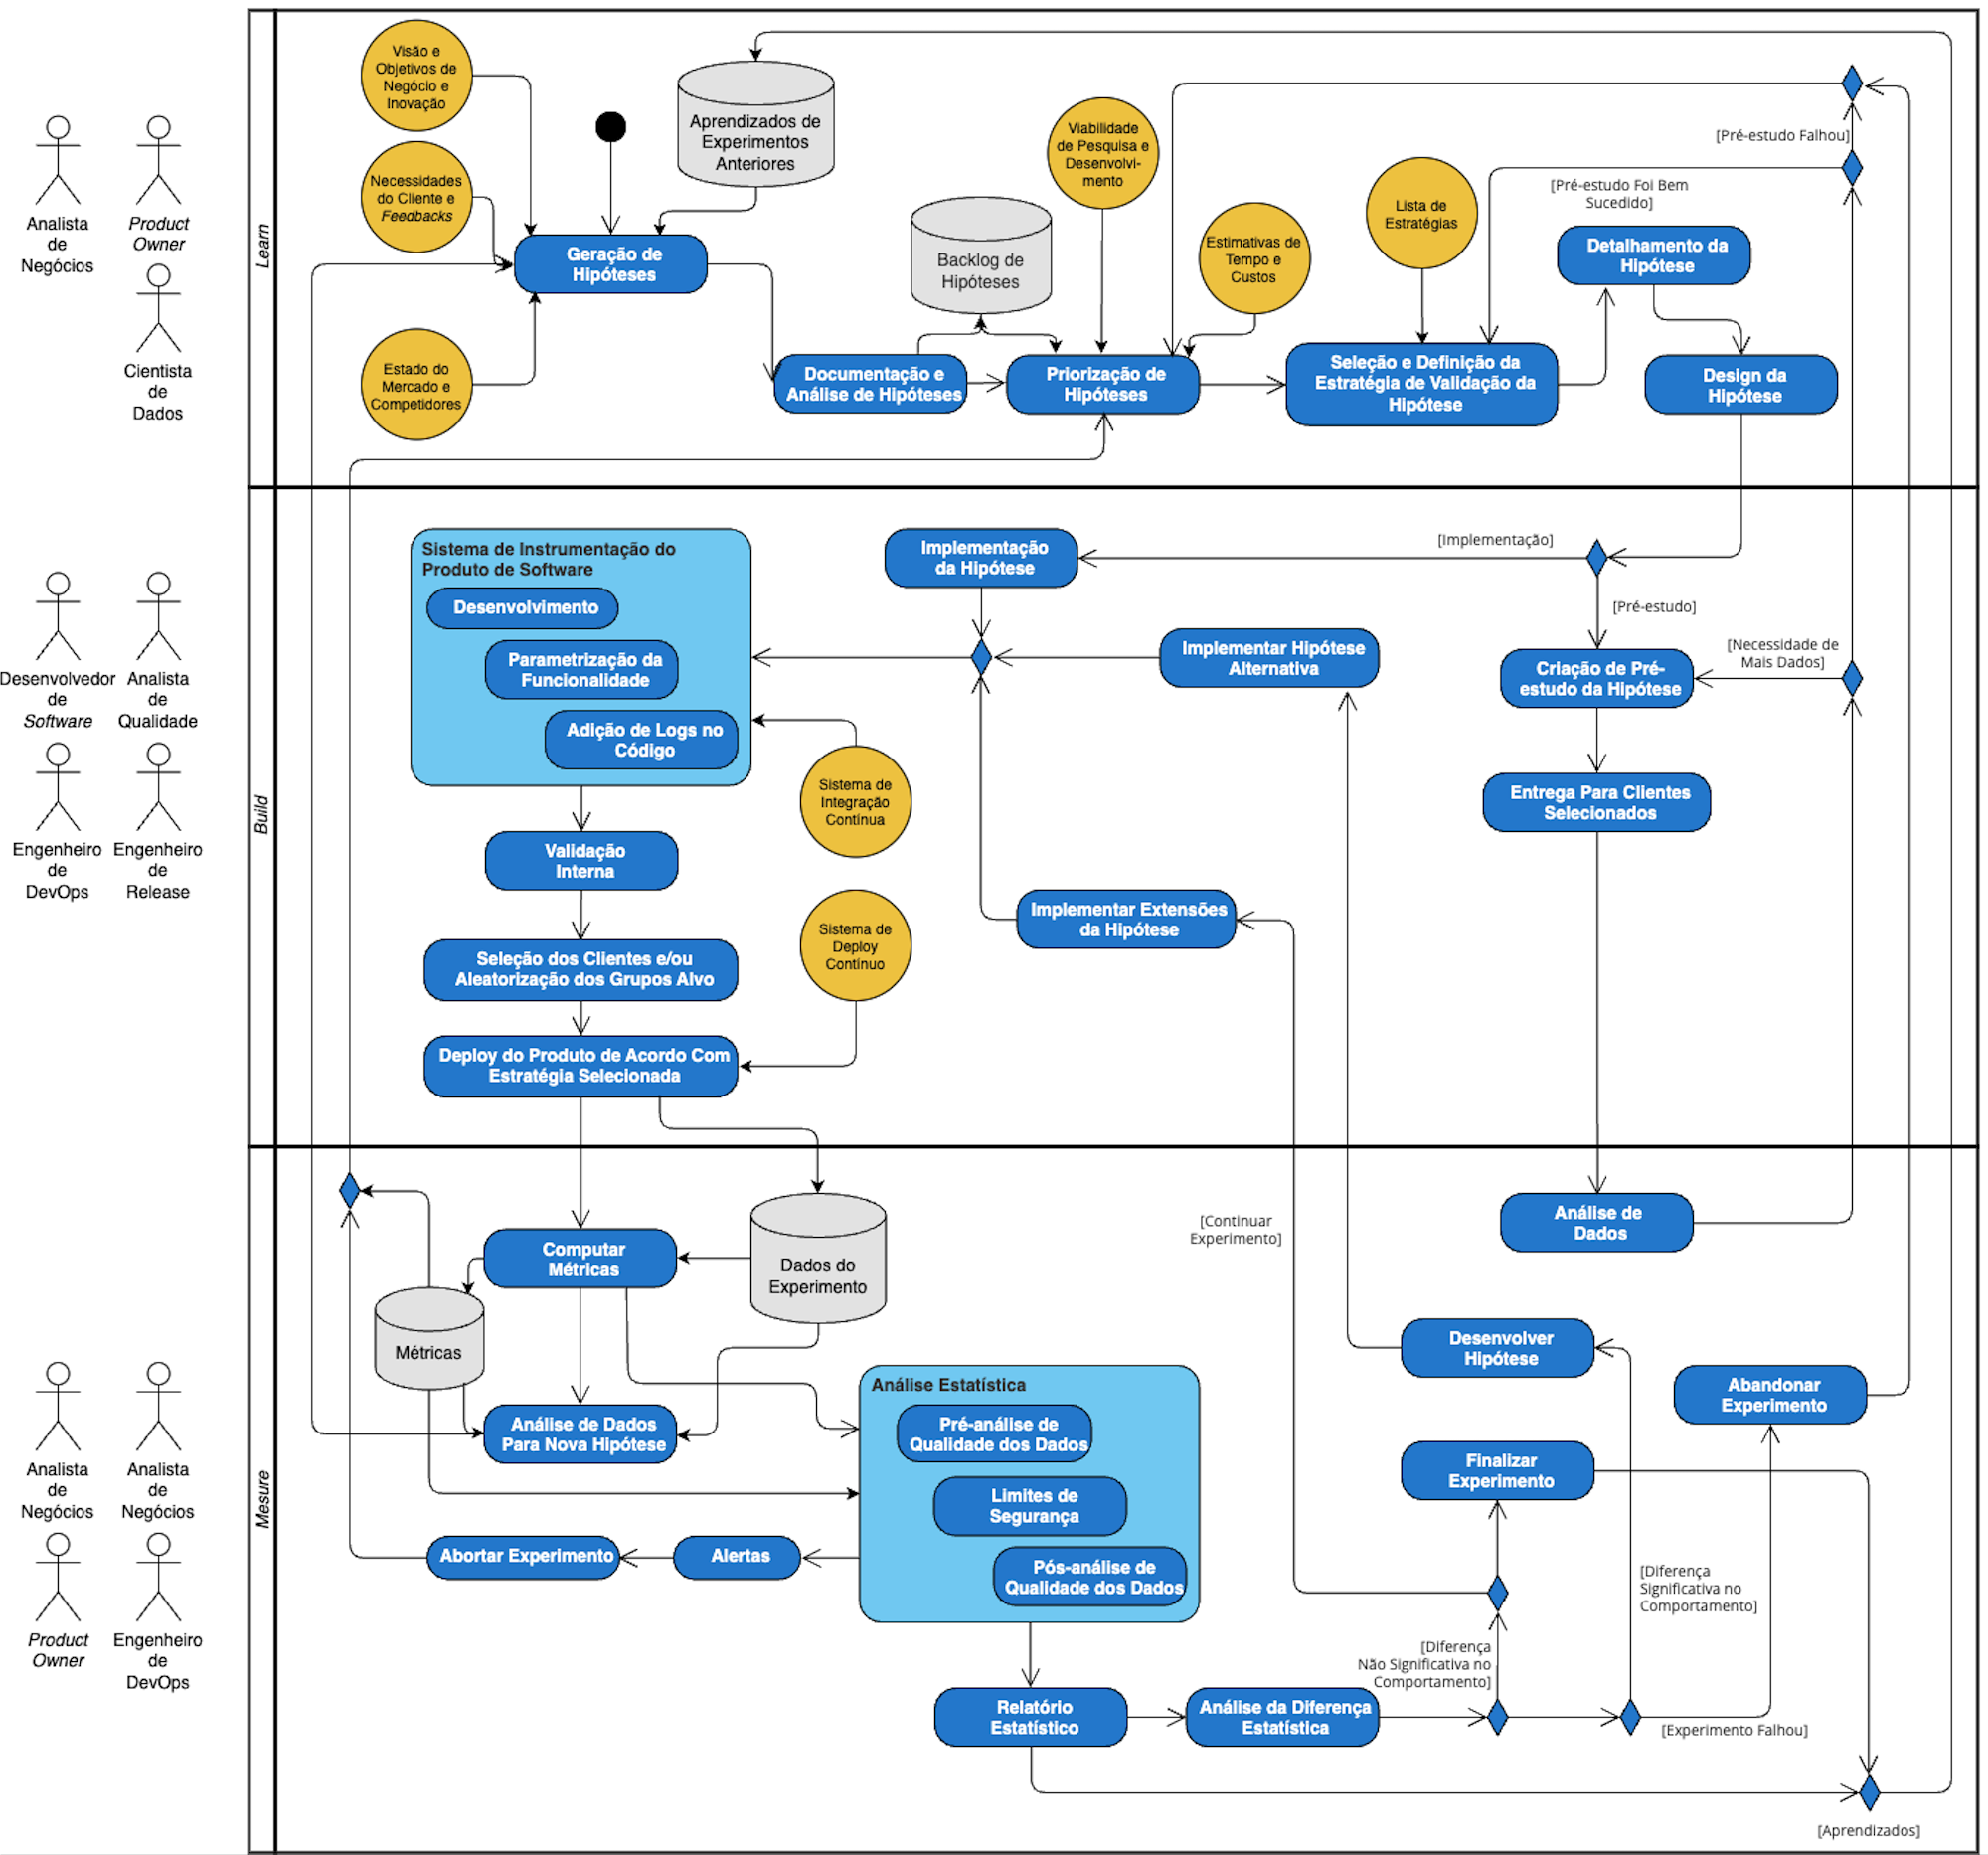
\includegraphics[width=1\linewidth]{figuras/combined_ce_process.png}
\text{Fonte: Adaptado de \citeonline{erthal_characterization_2023}}
\label{fig:erthal-process}
\end{figure}

% O artigo \citeonline{erthal_characterization_2023} realiza um trabalho minucioso na caracterização da literatura, trazendo diversos estudos primários e modelos já existentes. Por isso, o processo proposto pelos autores se apresenta como uma fonte confiável de referência. Desta forma, optou-se por guiar as atividades a serem realizadas no Estudo de Caso desta monografia a partir do modelo apresentado, analisando o processo de desenvolvimento atual do produto analisado e identificando atividades faltantes ou melhorias para as já existentes.

\section{Análise Estatística de Dados}
\label{sec:ref-analise-dados}

Esta seção aborda os conceitos e metodologias do domínio da estatística necessários para testes de hipótese. O propósito é realizar uma contextualização nas metodologias que serão empregadas durante a análise dos dados quantitativos durante o estudo de caso deste trabalho.

Para a realização de decisões estatísticas, são formuladas \textbf{hipóteses estatísticas}, que servem para guiar a avaliação de amostras de dados coletadas, bem como tomadas de decisão. Em um experimento, estas hipóteses são definidas na fase de planejamento e devem guiar todo o processo de experimentação. Quando desejamos analisar a diferença entre duas amostras, formulamos hipóteses para que as mesmas sejam aceitas ou rejeitadas, iniciando pela proposição de que não há diferença entre as amostras. Esta hipótese inicial é chamada de \textbf{hipótese nula}, já as demais são chamadas \textbf{hipóteses alternativas} \cite{juristo_basics_2001}.

Visando rejeitar a hipótese nula, se analisa a diferença entre as amostras coletadas e, caso esta seja considerável, entende-se que é \textit{significativa} e suficiente para a tomada de decisão. As maneiras pelas quais medimos este nível de diferença são chamadas de \textbf{testes de significância} ou \textbf{regras de decisão} \cite{juristo_basics_2001}.

Quando a hipótese nula é rejeitada quando não deveria, se caracteriza um \textbf{erro do tipo I}, ou seja, um falso positivo. Quando o contrário acontece e a hipótese nula é aceita quando não deveria, um falso negativo, se tem um \textbf{erro do tipo II}. O risco de acontecimento de ambos os erros podem ser mitigados através do aumento da amostra, porém, isso nem sempre é possivel \cite{wohlin_experimentation_2012}.

Ao se realizar um teste de hipótese, é definido um \textbf{nível de significância}, que seria o nível máximo que o pesquisador está disposto a arriscar cometer um erro de tipo I. Ou seja, caso seja definido um nível de 0.05 (5\%), é aceito que a cada 100 análises, 5 rejeitarão a hipótese nula quando ela deveria ser aceita. Normalmente este nível é representado pela letra grega alfa (\( \alpha \)) \cite{juristo_basics_2001}.

Já os erros de tipo II dependem de outros fatores, como a diferença nas observações das diferentes hipóteses e poder do teste estatístico, representada por beta (\( \beta \)). O \textbf{poder de um teste} é definido pela probabilidade de se rejeitar corretamente a hipótese nula, representado por 1 - \( \beta \). Por exemplo, um nível de poder de 0.4 indica que se um experimento for executado 10 vezes um efeito causado por algum fator alternativo será descoberto apenas em 4 delas \cite{juristo_basics_2001}.

\subsection{Estatística Descritiva}
\label{subsec:descritiva}

Após a coleta dos dados, pode se utilizar de métodos de estatística descritiva para se apresentar e descrever estes conjuntos, visando entender sua natureza e identificar anomalias. O objetivo é observar a distribuição do conjunto, se há dados que podem ser desconsiderados e decidir o teste de hipótese mais adequado para a comparação das amostras \cite{wohlin_experimentation_2012}.

\subsubsection{Medidas de Tendência Central e de Distribuição}

\citeonline{wohlin_experimentation_2012} definem que as medidas de tendência central visam apontar o centro do conjunto de dados, e que para isso utilizam os valores de \textbf{média (\( \overline{x} \))}, que é soma dos valores divida pela sua quantidade, \textbf{moda}, que se trata do valor mais recorrente do conjunto e \textbf{mediana (\( \tilde{x} \))}, que seria o valor encontrado no meio do conjunto após sua ordenação.

A mediana, também pode ser representada como \(x_{50\%}\), o que indica que ela é o percentil 50\%. Um \textbf{percentil} \(x_p\) indica o valor abaixo do qual \(p\%\) dos dados se encontram. Existem casos especiais de percentis chamados \textbf{quartis}, que dividem os dados em quatro partes iguais: o primeiro quartil (Q1 ou \(l_q\)) marca o valor abaixo do qual se encontra 25\% dos dados amostrais, e o terceiro quartil (Q3 ou \(u_q\)), 75\% \cite{wohlin_experimentation_2012}.

\citeonline{wohlin_experimentation_2012} também apresentam as medidas de distribuição, que por sua vez visam apresentar quão concentrado está o conjunto de dados. Para isto utiliza-se de medidas como a \textbf{variância (\textit{\( s^2 \)})}, o \textbf{desvio padrão (\textit{s})} e a \textbf{amplitude}. A amplitude é a distância entre os valores máximos e mínimos do conjunto. A variância é a média dos quadrados das distâncias entre os valores da amostra e sua média. O desvio padrão é a raiz quadrada da variância. Então, sendo \textit{s} o desvio padrão, \( s^2 \) a variância, \textit{n} o número de dados observados e \(x_i \) o i-ésimo dado observado, as medidas citadas podem ser representadas da seguinte forma:
\[
\text{amplitude} = x_{\text{max}} - x_{\text{min}}
\]

\[
\textit{s} = \sqrt{s^2}
\]

\[
s^2 = \frac{1}{n} \sum_{i=1}^{n} (x_i - \bar{x})^2
\]


\subsubsection{Representação Gráfica}

Além das medidas existentes na estatística descritiva, \citeonline{wohlin_experimentation_2012} também abordam como a representação gráfica do conjunto de dados pode ajudar a entender a natureza do conjunto, ajudando a identificar visualmente \textit{outliers}, que são pontos que diferem muito do conjunto e atrapalhar a análise. Os autores apresentam diferentes tipos de gráficos que podem ser úteis para esta prática, alguns deles são:

\begin{itemize}
    \item \textbf{Gráfico de Dispersão:} apresenta amostras pareadas em duas dimensões, permitindo identificar dependências, padrões lineares e \textit{outliers} (exemplificado na Figura \ref{fig:scatterplot});
    \item \textbf{Gráfico de Caixa (\textit{Box Plot}):} permite se visualizar a dispersão e a assimetria dos dados. Apresenta a mediana, o primeiro e o terceiro quartis (exemplificado na Figura \ref{fig:boxplot}). A largura da caixa é \textit{d} onde \textit{d} = \(u_q\) - \(l_q\). O gráfico é delimitado por suas caudas (ou bigodes), que se estendem até 1,5 vezes o comprimento da caixa a partir dos quartis. Esta delimitação serve para representar a área onde, teoricamente, todos os dados conjunto deveriam ser encontrados, ou seja, aqueles fora desta região são considerados \textit{outliers}; e
    \item \textbf{Histograma:} representa a distribuição dos dados e mostra a frequência de intervalos de valores (exemplificado na Figura \ref{fig:histogram}). Cada barra representa a quantidade de dados dentro de um intervalo específico e sua altura indica a frequência de dados dentro deste intervalo. Isto permite observar facilmente a distribuição que os dados seguem ou se existem picos ou lacunas significativas.
\end{itemize}

\begin{figure}
    \centering
    
    \caption{Exemplo de Gráfico de Dispersão}
    
    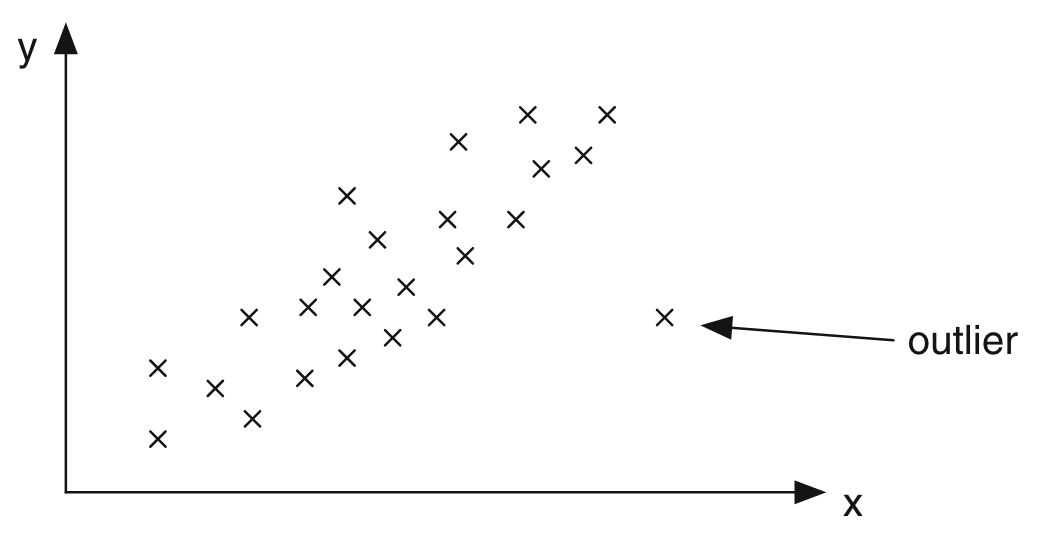
\includegraphics[width=0.7\linewidth]{figuras/scatter.png}
    
    \text{Fonte: \citeonline{wohlin_experimentation_2012}}
    
    \label{fig:scatterplot}
\end{figure}

\begin{figure}
    \centering
    
    \caption{Exemplo de Gráfico de Caixa}
    
    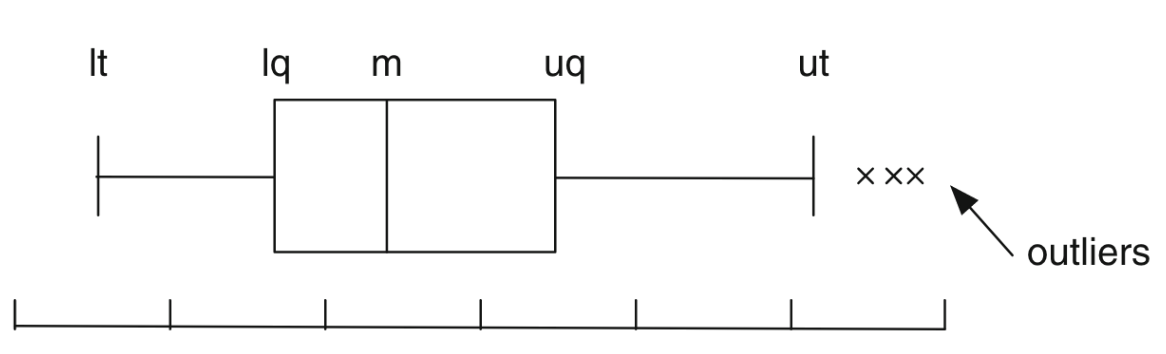
\includegraphics[width=0.7\linewidth]{figuras/boxplot.png}
    
    \text{Fonte: \citeonline{wohlin_experimentation_2012}}
    
    \label{fig:boxplot}
\end{figure}

\begin{figure}
    \centering
    
    \caption{Exemplo de Histograma}
    
    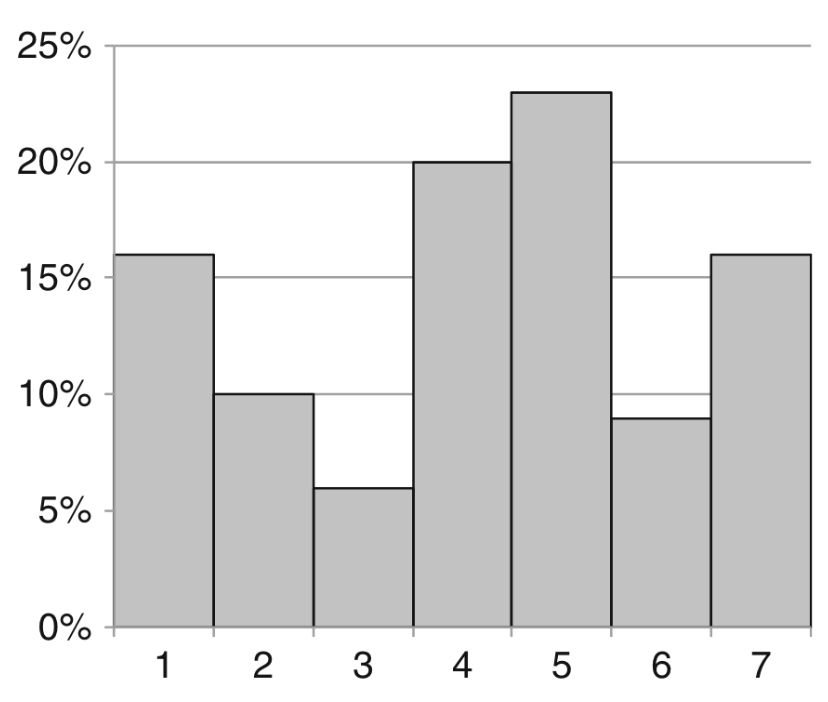
\includegraphics[width=0.5\linewidth]{figuras/histogram.png}
    
    \text{Fonte: \citeonline{wohlin_experimentation_2012}}
    
    \label{fig:histogram}
\end{figure}

A identificação dos \textit{outliers} por meio destes processos de representação gráfica é crucial para a chamada \textbf{redução dos dados}. Valores que se desviam significativamente dos demais podem comprometer a qualidade do conjunto de dados e prejudicar a análise. Portanto, é fundamental identificá-los e avaliar a necessidade de sua remoção. Caso um valor resulte de um evento raro, ele pode ser removido; no entanto, um ponto que revele informações valiosas deve ser analisado separadamente \cite{wohlin_experimentation_2012}.

\subsection{Teste de Hipóteses}

O objetivo de um teste de hipótese é verificar se é possível rejeitar uma hipótese nula a partir da análise de um determinado conjunto de dados. Ou seja, \(x_i \) descreve determinadas propriedades e o teste visa negar estas características com determinado nível de significância \cite{wohlin_experimentation_2012}. 

Um teste de hipótese pode ser paramétrico ou não paramétrico. Os paramétricos se baseiam em modelos que pressupõem a distribuição dos dados coletados, já os não paramétricos não fazem suposições \cite{juristo_basics_2001}. Um destes pressupostos pode ser que o conjunto está normalmente distribuído. Esta distribuição é caracterizada por uma curva simétrica em formato de sino e isso pode ser verificado através de diferentes tipos de gráficos \cite{wohlin_experimentation_2012}.

A seguir serão apresentados alguns testes de hipótese existentes, métodos que se adequam ao contexto deste trabalho, onde serão avaliadas amostras independentes de dados, que podem ser grandes ou pequenas e que podem ter sua distribuição normal ou não.

\subsubsection{Teste Z}

Este é um teste paramétrico para quando trabalhamos com amostras grandes (\(n \geq 30\)). Nestes conjuntos a distribuição das médias amostrais tende a ser normal, o que significa que a média das amostras se aproxima da média da população total, assim como o desvio padrão. Isso facilita a inferência sobre a população total com base nos dados coletados \cite{juristo_basics_2001}.

Utiliza-se da regra de decisão de diferença entre médias para se avaliar a significância da diferença entre as duas amostras coletadas. Caso essa diferença não seja significativa, se entende que a diferença observada pode ser atribuída ao acaso, o que nos leva a não rejeitar a hipótese nula. O valor responsável por nos dizer o valor dessa significância é chamada de z (ou \textit{z-score}) \cite{juristo_basics_2001}.

\citeonline{juristo_basics_2001} demonstram que para calcular o valor de \textit{z}, primeiro realizamos um processo de normalização dos valores da amostra analisada, para que possamos distribuir nossos dados na distribuição padrão da variável \textit{z}, apresentada na Figura \ref{fig:z-score} (onde a média é 0 e o desvio padrão é 1). Nesta curva, o valor central é 0, e o eixo x tem como medida o desvio padrão, que no caso é 1, o valor de \textit{z} vai nos dizer quantos desvios padrões um dado valor se distancia da média, que é 0. 

Para calcular o valor de \textit{z} se utiliza a seguinte fórmula, onde \textit{S} é alguma medida da amostra (média, desvio padrão, etc), e \(\mu_S\) e \(\sigma_S\) são respectivamente a média e o desvio padrão desta medida:

\[
z = \frac{S - \mu_S}{\sigma_S}
\]

Assim, os valores mais distantes se encontram nas regiões críticas, como apresentado na Figure \ref{fig:z-score}, que demonstra que os valores encontrados nelas teriam um \textit{z-score} maior que 1.96 ou menor que -1.96 (no exemplo o nível de significância é de 0.05, ou 5\%).



\begin{figure}
    \centering
    
    \caption{Distribuição da Estatística Z}
    
    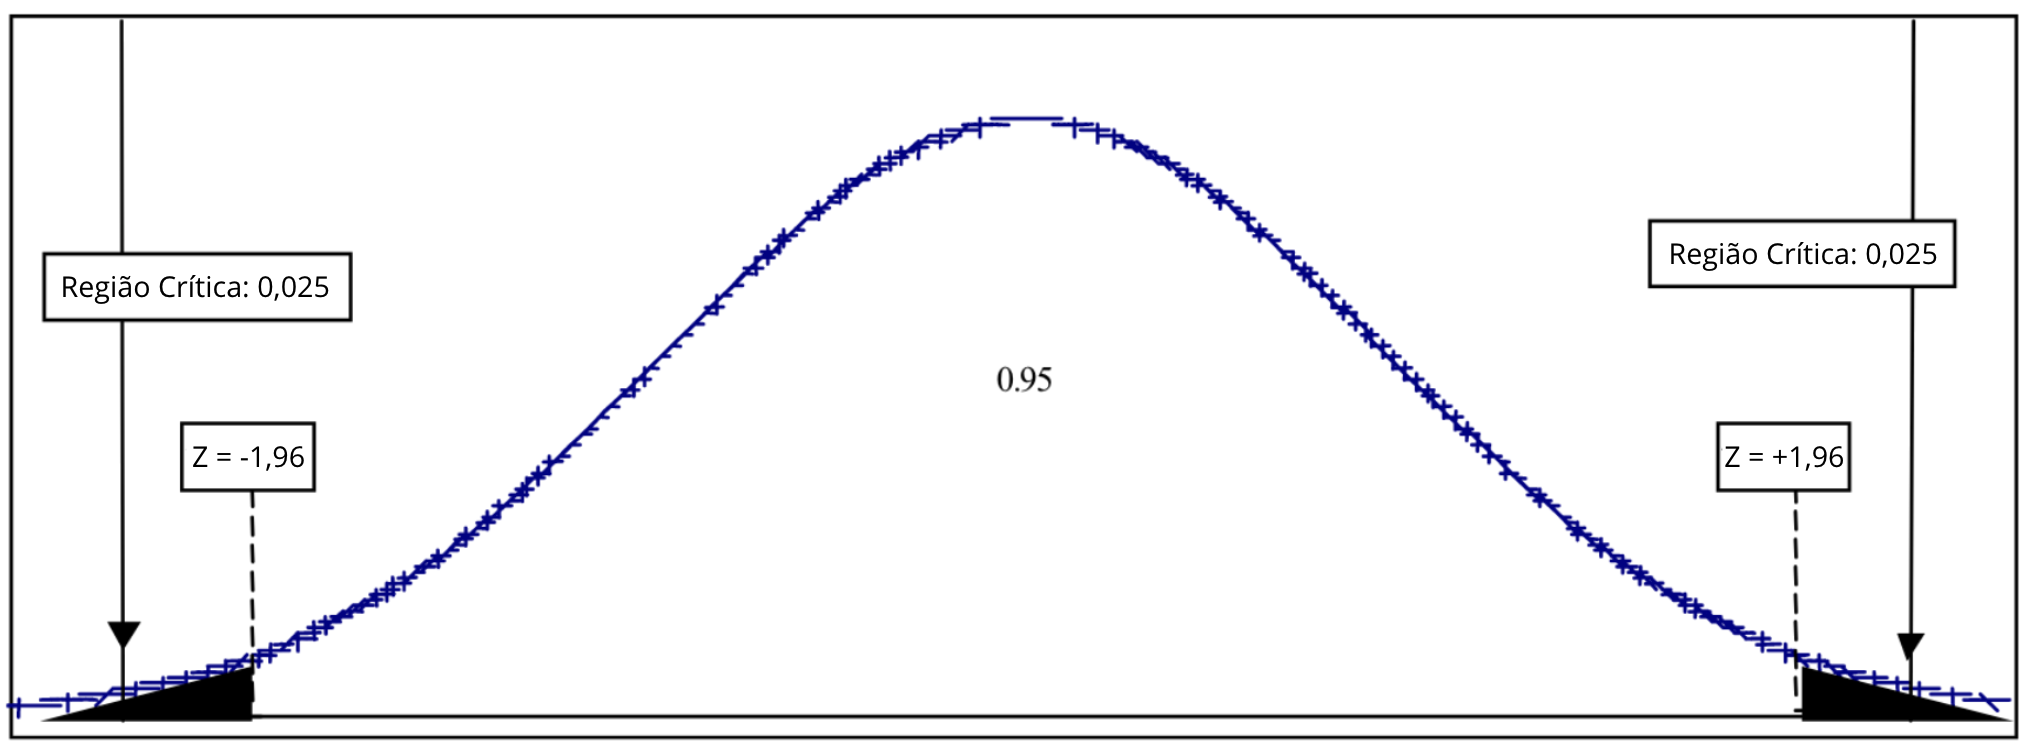
\includegraphics[width=1\linewidth]{figuras/z_distr.png}
    
    \text{Fonte: Adaptado de \citeonline{juristo_basics_2001}}
    
    \label{fig:z-score}
\end{figure}

\subsubsection{Teste T de Student}
\label{subsec:t-test}

Este também é um teste paramétrico, onde se espera que a amostra coletada se aproxime da distribuição normal. É uma alternativa para quando se lida com conjuntos pequenos de dados. A distribuição do valor de \textit{t} é bem parecida com a distribuição normal, porém depende do grau de liberdade da amostra, que é representado por \textit{v}. Quanto maior o grau de liberdade, mais a curva da distribuição se aproxima da curva normal \cite{juristo_basics_2001}. Esse teste é comumente utilizado para comparar duas amostras independentes de variáveis numéricas \cite{wohlin_experimentation_2012}.

A curtose é uma característica da estatística descritiva que define o achatamento da curva de uma distribuição. A curtose de uma distribuição normal é 0, indicando uma distribuição com um formato de sino padrão. Em contraste, a curtose de uma distribuição t de Student tende a ser cada vez mais negativa conforme o grau de liberdade diminui \cite{juristo_basics_2001}. Isso significa que, com menos graus de liberdade, a distribuição t apresenta caudas mais largas e uma forma mais achatada, refletindo a maior variabilidade e incerteza associadas a amostras menores, vide a Figura\ref{fig:t-statistic}.

O grau de liberdade é calculado a partir da quantidade de amostras a serem testadas e seus respectivos tamanhos, sendo uma amostra \textit{v} = \textit{n} - 1, para duas amostras \textit{v} = \textit{\(n_1\)} + \textit{\(n_2\)} - 2 e assim sucessivamente \cite{juristo_basics_2001}.



\begin{figure}
    \centering
    
    \caption{Distribuição de T Para Diferentes Graus de Liberdade}
    
    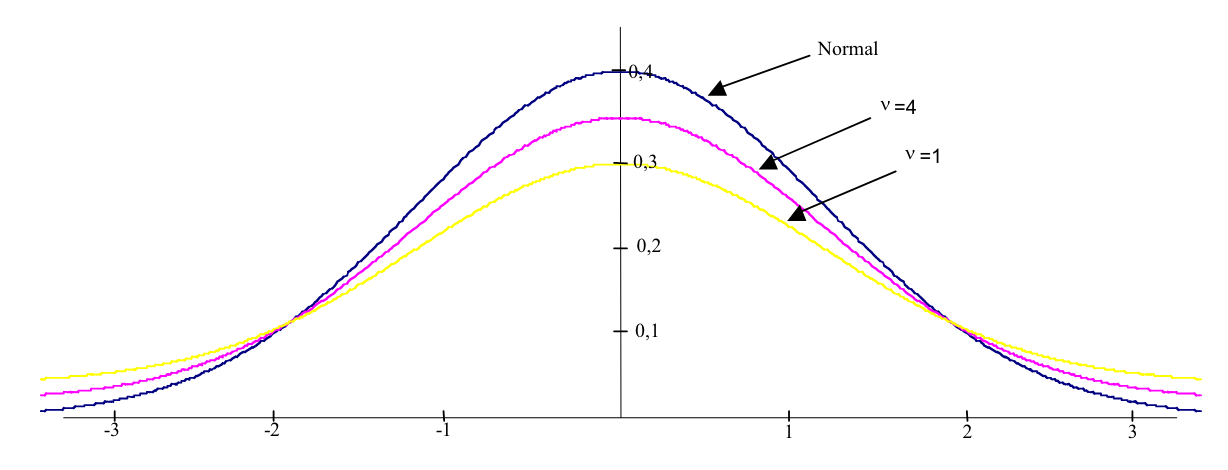
\includegraphics[width=1\linewidth]{figuras/t-statistic.png}
    
    \text{Fonte: \citeonline{juristo_basics_2001}}
    
    \label{fig:t-statistic}
\end{figure}


Para se calcular o valor \textit{t} utiliza-se a fórmula:

\[
t = \frac{\bar{x} - \mu}{s / \sqrt{n}}
\]

onde \(\bar{x}\) é a média amostral, \(\mu\) é a média da população (ou a média de outra amostra), \(s\) é o desvio padrão amostral e \(n\) é o tamanho da amostra. O valor calculado de t é então comparado com os valores críticos da tabela t, que são ajustados para diferentes níveis de significância e graus de liberdade. Esses valores críticos ajudam a determinar se a diferença observada é estatisticamente significativa. A tabela t de Student é gerada a partir de cálculos que levam em consideração a distribuição das amostras \cite{juristo_basics_2001}.




\subsubsection{Teste de Mann-Whitney U}
\label{subsec:u-test}

O teste de Mann-Whitney U, também conhecido como teste U, é uma alternativa não paramétrica para a análise de duas amostras. Este teste não assume que os dados seguem uma distribuição normal, tornando-o mais flexível e aplicável a dados medidos em escalas ordinais. O teste é utilizado para determinar se há uma diferença significativa entre duas amostras independentes \cite{wohlin_experimentation_2012}.

\citeonline{juristo_basics_2001} demonstram que para se realizar o teste de Mann-Whitney U, as observações das duas amostras são organizadas em ordem crescente e substituídas pelos seus postos ou \textit{ranks}. Quando há empates, cada valor é substituído pela média dos \textit{ranks} correspondentes. A soma dos \textit{ranks} para cada amostra é calculada e utilizada para determinar o valor da estatística \textit{u}. A fórmula para o cálculo de \textit{u} é:

\[
u = r_1 - \frac{n_1 (n_1 + 1)}{2}
\]

onde \(r_1\) é a soma dos \textit{ranks} da primeira amostra e \(n_1\) é o número de observações na primeira amostra. A distribuição amostral de \(u\) é simétrica e, quando o tamanho das amostras é suficientemente grande (geralmente \(n_1 \geq 8\) e \(n_2 \geq 8\)), a distribuição de \(u\) pode ser aproximada por uma distribuição normal com média (\(\bar{x}\)) e variância (\textit{s}) dadas por:

\[
\bar{x} = \frac{N_1 N_2}{2}
\]
\[
\text{s} = \frac{n_1 n_2 (n_1 + n_2 + 1)}{12}
\]

O valor \(z\) é calculado como:

\[
z = \frac{u - \bar{x}}{s}
\]

Esse valor \(z\) é então comparado com os valores críticos da tabela padrão normal para determinar se a diferença observada entre as amostras é estatisticamente significativa. Se \(z\) cair fora do intervalo crítico definido (por exemplo, -1.96 a 1.96 para um nível de significância de 0.05), rejeita-se a hipótese nula e conclui-se que há uma diferença significativa entre as amostras \cite{juristo_basics_2001}.

\subsubsection{Teste Qui-Quadrado}
\label{subsec:chi-square}

O teste qui-quadrado também é um teste não paramétrico. É utilizado para analisar a diferença entre as frequências observadas e esperadas de uma variável categórica. O objetivo do teste é verificar se há uma diferença significativa entre as frequências esperadas, sob uma hipótese nula \(h_0\), e as frequências observadas. É um teste indicado para amostras grandes, diferindo do Mann-Whitney, que é mais apropriado para amostras pequenas \cite{juristo_basics_2001}. Para realização deste teste se utiliza a estatística qui-quadrado (\(\chi^2\)), que é calculada usando a seguinte fórmula:

\[
\chi^2 = \sum_{i=1}^{k} \frac{(o_i - e_i)^2}{e_i}
\]

onde \(o_i\) são as frequências observadas, \(e_i\) são as frequências esperadas sob a hipótese nula, e \(k\) é o número de eventos ou categorias. O valor calculado de \(\chi^2\) é então comparado a um valor crítico da tabela qui-quadrado, que varia de acordo com o número de graus de liberdade (\(\nu = k - 1\)) e o nível de significância escolhido \cite{juristo_basics_2001}.

Se o valor calculado de \(\chi^2\) for maior que o valor crítico da tabela (como \(\chi^2_{0.95}\), para um nível de significância de 0,05), a hipótese nula é rejeitada, indicando uma diferença significativa entre as frequências observadas e esperadas. Caso contrário, não há evidência suficiente para rejeitar a hipótese nula \cite{juristo_basics_2001}.


\section{Resumo do Capítulo}

Este capítulo abordou os principais conceitos utilizados no desenvolvimento deste estudo, incluindo as metodologias de pesquisa, os modelos nos quais a proposta do estudo se baseou, bem como as arquiteturas e técnicas escolhidas para sua implementação. Dentre estas se destacam as \textit{feature toggles} e os conceitos e métodos estatísticos que fundamentarão os testes de hipótese à serem realizados.

Além disso, foram conceituadas e apresentadas as estratégias de investigação a utilizadas neste trabalho, como a Revisão Sistemática da Literatura, que orientou o estudo realizado para desenvolvimento deste trabalho, o Estudo de Caso, cujos processos serão executados na segunda fase desta monografia, e, por fim, o Experimento, que é o principal objeto do processo proposto de experimentação contínua.

Com base em normas técnicas, também foram caracterizadas a qualidade do \textit{software} e a qualidade em uso. Essas normas apresentam critérios e diretrizes para avaliar a qualidade de um produto de \textit{software}, os quais estão diretamente relacionados aos experimentos, que têm como objetivo aumentar e assegurar a qualidade de um sistema.
